\fancychapter{User Studies}
\label{chap:userstudies}

The developed rapport system was tested in collaboration with Nuno Xu, who is studying the impact of perceived task performance on trust. Using the Quick Numbers scenario (Figure~\ref{fig:quickNumbersScenario} and \ref{fig:quickNumbersScenarioCloseup}), we evaluate how both task performance and willingness would jointly affect trust, and observe its impact on rapport using robot \ac{EMYS}. This thesis focus only on the rapport aspects of the study, therefore, please consult Xu's Master's thesis for more details regarding how trust is evaluated~\cite{Xu2016}.

\begin{figure}[H]
	\centering
	\frame{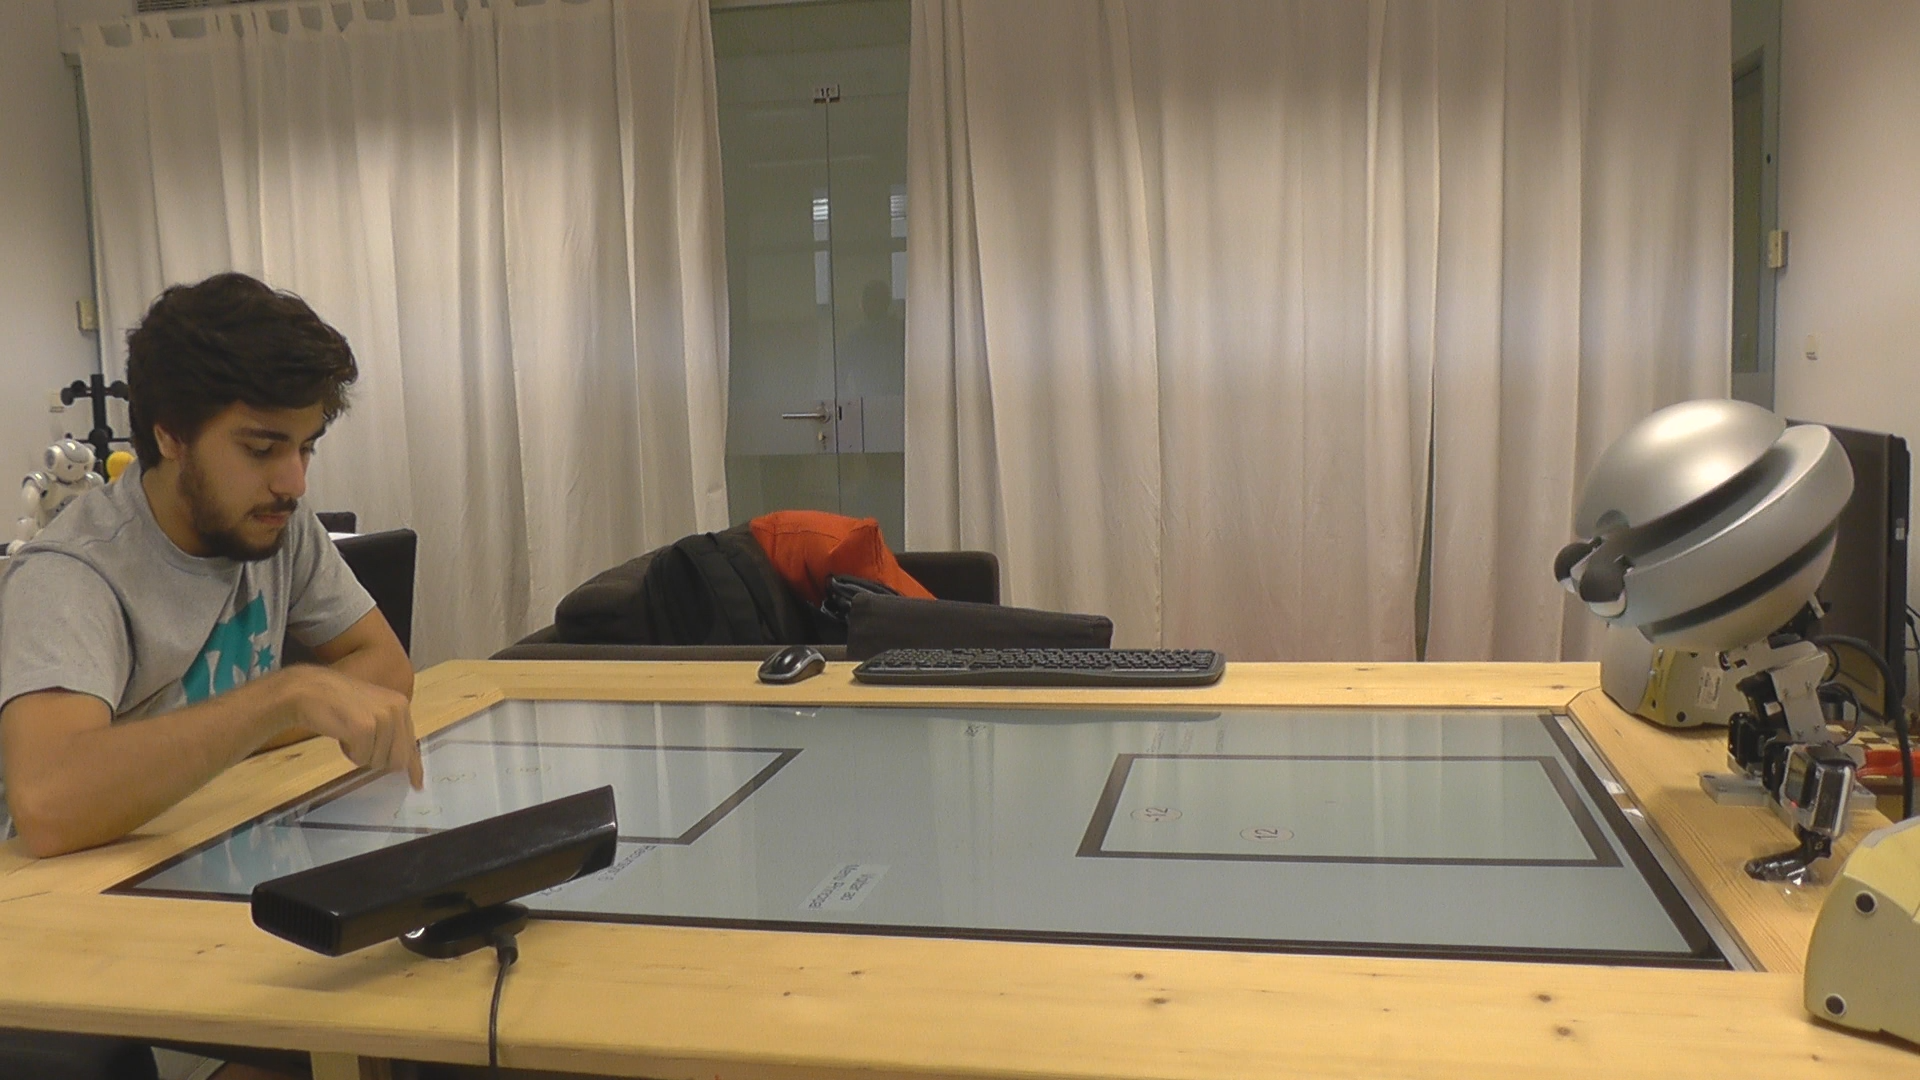
\includegraphics[width=0.7\textwidth]{images/ScenarioScreenShot.png}}
	\caption{An example of a participation in the Quick Numbers study (side view).}
	\label{fig:quickNumbersScenario}
\end{figure}

\section{Quick Numbers}
\label{sec:ScenarioDescription}

In the Quick Numbers scenario players are tasked with gaining as many resources as possible within the given time by interacting with a touch table. At the beginning, each player starts with a fixed amount of resources that can be invested before each round. Depending on the amount invested and the player's performance, the returning investment will either be greater or lesser than the investment. The task is to tap the appearing numbers in sequential order starting with number one until the end of the round (Figure~\ref{fig:quickNumbers}). With each successful tap, the score increases, and with each incorrect number, the score decreases. In the end, the resources earned are the product between the amount invested and the round's score.

In this study, \ac{EMYS} accompanies the subject throughout the scenario, not as an opponent, but as another player that is also playing the game. The scenario stages go as follow:
\begin{itemize}
	\item \textbf{Introduction}: researchers briefly explains the scenario procedures, followed by the start the scenario, where the agent starts by greeting the participant;
	\item \textbf{Training Stage}: the participant plays an informal match alone to get accustomed to the game mechanics before proceeding;
	\item \textbf{Gaming Session}: both players play a single round, at the same time;
	\item \textbf{Results Discussion}: the agent comments each player score;
	\item \textbf{Investment}: the participant is informed that he has to invest on the agent. The participant is unaware how much the agent will give in return;
	\item \textbf{Ending}: \ac{EMYS} informs the value of the investment return and thanks to the subject for his participation.	
\end{itemize}

\begin{figure}[H]
	\centering
	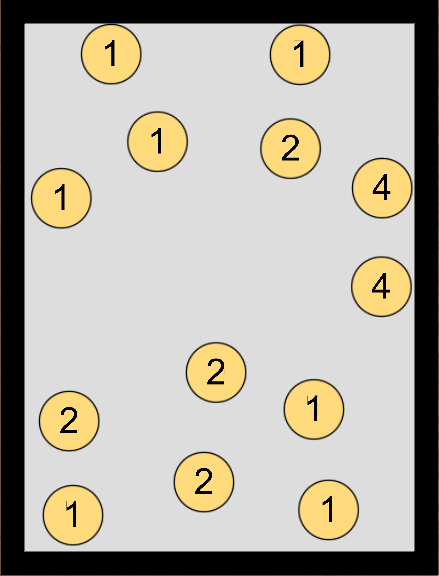
\includegraphics[width=0.3\textwidth]{images/FallingBoltsDiagram.png}
	\caption{Illustration of the Quick Numbers game developed in Unity.}
	\label{fig:quickNumbers}
\end{figure}

\section{Quick Numbers Plugins}

In addition to the plugins that implements the rapport model, we developed the following:
\begin{itemize}
	\item \textbf{Scenario \textit{Perceiver}}: monitors the scenario through \textit{Thalamus}, notifying the interested \textit{Effectors} regarding the current state of the scenario. For example, it notifies \textit{Effectors} whenever the participant tapped the correct number;
	\item \textbf{Utterances Manager}: proposes utterances according to the dyadic state of the interaction;
	\item \textbf{Rapport Strategies Manager}: enables/disables the rapport \textit{Effectors} given the current state of the interaction; 
\end{itemize}

\subsection{Utterances Manager}

This \textit{Effector} implements the positivity and the coordination component of the rapport model as it proposes utterances (in Portuguese) according to the dyadic state of the interaction following the same structure as Table~\ref{fig:extended:utterances} (Appendix D). In addition, the agent greets and dismisses properly at the beginning and at the end of the interaction, respectively, however, the rapport agent is friendlier. For example, as detailed in rapport model (Chapter~\ref{chap:rapportModel}), the rapport agent shares a personal information when introducing itself, and will motivate or praise the agent's performance. Furthermore, and more importantly, given that the participant speaks Portuguese, \ac{EMYS} will adapt his utterances according to the participant's gender. To sum up, the rapport agent:

\begin{itemize}
	\item Shares a personal information when introducing itself - ``Did you know I played Sueca recently?''~\cite{correia2016trust};
	\item Is friendlier and more comprehensive by motivating and praising the participant's performance - ``You are doing great!'', ``Don't worry, I also had a rough start'';
	\item Shows embarrassment when hitting the wrong number - ``Today's not my day'';
	\item Attempts to be humorous - ``I just finished. I won't go anywhere... how could I? I am just a head...''.
\end{itemize}

Appendix D contains the full list of the utterances used in conditions C and R for male participants.

\subsection{Rapport Strategies Manager}

The Rapport Strategies Manager \textit{Effector} defines which rapport strategies are active given the current stage of the scenario. For example, following Table~\ref{table:enabledPlugins}, it disables postural mimicry and mutual gaze rapport strategies when \ac{EMYS} participates in Quick Numbers as a player and not as a spectator. In particular, it disables Facial Expression Mimicry \textit{Effector} in the investment phase because the participant's face is not visible on the video feed (Section~\ref{sub:sec:FacialExpressionMimicry}).

\begin{table}[H]
	\centering
	\begin{tabular}{|l|c|c|c|}
	\hline
	\multicolumn{1}{|c|}{\textbf{Scenario Stage}} & \textbf{Facial Expression Mimicry} & \textbf{Head Gesture Mimicry} & \textbf{Mutual-Gaze} \\ \hline
	Introduction & \cmark & \cmark & \cmark (Between-tasks) \\ \hline
	Training Stage & \cmark & \cmark & \cmark (In-tasks) \\ \hline
	Gaming Session & \xmark & \xmark & \xmark \\ \hline
	Results Discussion & \cmark & \cmark & \cmark (Between-tasks) \\ \hline
	Investment & \xmark & \xmark & \xmark \\ \hline
	Ending & \cmark & \cmark & \cmark (Between-tasks) \\ \hline
	\end{tabular}
	\caption{Rapport strategies presence throughout the different stages of the Quick Numbers scenario.}
	\label{table:enabledPlugins}
\end{table}

\section{Methodologies and Procedures}
\label{sec:methodsAndProcedures}

In order to study the impact of the three components of rapport on users using a robotic agent we conducted a between-subjects study using the Quick Numbers scenario, following two conditions:

\begin{itemize}
	\item \textbf{Condition C:} the agent does not attempt to build rapport;
	\item \textbf{Condition R:} the agent attempts to build rapport using the rapport model described in Chapter~\ref{chap:rapportModel}.
\end{itemize}

In addition, as the study was conducted in collaboration with Nuno Xu, we had two additional conditions that are outside of the scope of this dissertation:
\begin{itemize}
	\item \textbf{Condition T:} the agent does not attempt to build rapport but attempts to build trust~\cite{Xu2016};
	\item \textbf{Condition RT:} the agent attempts to build rapport and trust with the participant~\cite{Xu2016}.
\end{itemize}

In conditions C and R, the return value is always the agent's score multiplied by the participant's investment value, but this fact is unknown to the participant. In addition, the agent's \ac{AI} that plays the Quick Numbers game is identical in every condition. Specifically, the \ac{AI}'s performance was designed so that it had a reaction time of 0.3 seconds~\cite{Boot2008} and an accuracy of 70\% (empirically chosen value), so that the agent's does not perform necessary better than the participant which could make him frustrated.

Each participant answered the questionnaire available in Appendix A that is divided into three parts: the first part is answered before the participant interacts with \ac{EMYS}; the second part is filled during the investment stage while \ac{EMYS} plays alone; the last part is filled at the end of the scenario. The first questionnaire asks demographic information and if the participant had interacted with \ac{EMYS} in the past. The first and the second part aims to gather information regarding trust~\cite{carrington2007toward, schaefer2013perception}. The third part collects information to understand the participant's opinion regarding likeability, intelligence, and animacy using the Godspeed series~\cite{bartneck2009measurement, lehmann2015good} and 6-item scales (1 means low perception and 6 the highest level of perception). In addition, this part collects the participant's perception of proximity that we are attempting to increase by building rapport~\cite{aron1992inclusion} using a 7-item scale question (1 means that the participant did not feel close to the agent and 7 means that he felt very close).

Lastly, the user study sessions were individual and performed in an isolated room accompanied only by the researcher, and lasted between 20 and 30 minutes. The sessions were recorded using two cameras: one captured the participant from the front (Figure~\ref{fig:quickNumbersScenarioCloseup}) and the other captured the both \ac{EMYS} and the user (Figure~\ref{fig:quickNumbersScenario}).

\section{Sample Description}
\label{sec:sample}

A group of 40 participants from different universities campus were included in this study. The participants were equally selected and randomly distributed between the control condition (C) and the rapport condition (R). Condition C has a mean age of 23.5±1, equal distribution of genders, and over 55\% of the participants already interacted with \ac{EMYS}. Condition R has a mean age of 25.65±3.945, 60\% male and only 25\% of the sample played with \ac{EMYS} in the past.

\section{Results}

The main goal of the agent is to build rapport, therefore we raised the following hypothesis:
\begin{itemize}
	\item Are the rapport strategies effective in making agents more likeable?
	\item Does the developed system improve agent's liveness?
	\item Do rapport strategies affect perceived intelligence?
	\item Are the rapport strategies effective in establishing closer relationships between humans and agents?
\end{itemize}

All statistical analyses further mentioned used a significance level ($sig$) of 5\%.

%TODO PREP TALK
%In the attempt of answering these questions we will look compare the obtained results from the participants on both conditions. In addition to analysing the significance level, we will assess if there is a pattern that can be confi of the The results take into account both the significance level onto the significance level between the the control condition (C) and the rapport condition (R), and we will analyse
%In order to answer the first three questions, we used the information gathered from Godspeed questionnaires~\cite{bartneck2009measurement}, and the last from proximity questions~\cite{lehmann2015good, aron1992inclusion}. The document will firstly answer the above questions, ending with a brief discussion of the results.

\subsection*{\textit{Are the rapport strategies effective in making agents more likeable?}}

In order to infer a conclusion about this questions, we compared the likeability statistics between the control condition (Figure~\ref{fig:likeability_baseline}) and the rapport condition (Figure~\ref{fig:likeability_rapport}). As the distributions do not follow a normal distribution on both conditions ($sig_C=0.001$ and $sig_R=0$), and the groups are independent, we analyse the results using the \textit{Mann–Whitney U} statistical test. As the histogram's shapes are dissimilar ($sig=0.201$), we can only compare the mean scores: 5.0±0.649 and 5.3±0.865, on conditions C and R, respectively.

\begin{figure}[H]
	\centering
	\begin{minipage}[b]{.45\textwidth}
		\centering
		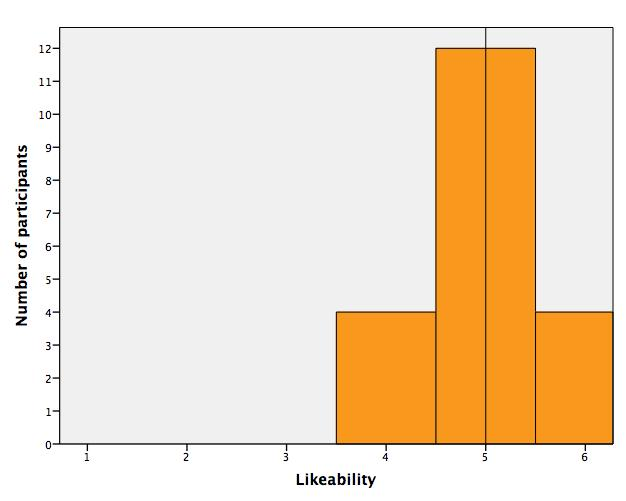
\includegraphics[width=\textwidth]{images/LikabilityBaseline.jpeg}
		\caption{Likeability histogram in the control condition. The vertical reference line marks the mean average of 5.0±0.649.}
		\label{fig:likeability_baseline}
	\end{minipage}
	\hfill
	\begin{minipage}[b]{.45\textwidth}
		\centering
		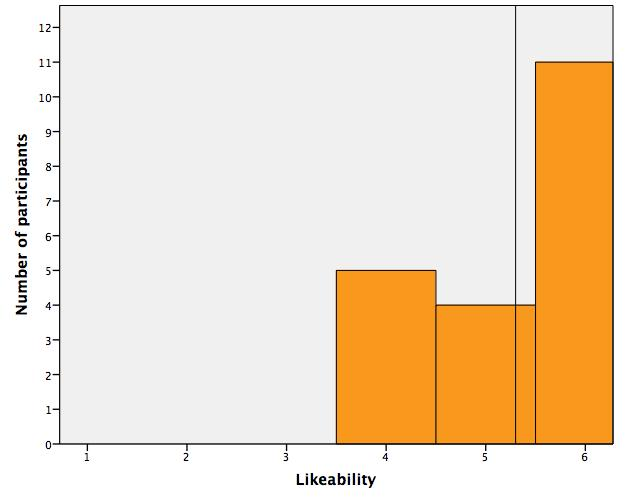
\includegraphics[width=\textwidth]{images/LikabilityRapport.jpeg}
		\caption{Likeability histogram in the rapport condition. The vertical reference line marks the mean average of 5.3±0.865.}
		\label{fig:likeability_rapport}
	\end{minipage}
\end{figure}

\textbf{Answer}: Despite the greater man average on the rapport condition, there is no statistical proof that rapport strategies are effective on increasing likeability. However, given that the mode (most frequent value) changed from 5 to 6, from condition C to condition R, we can postulate that, if we increase the sample size, we might obtain a clear confirmation that the rapport strategies affect the agent's likeability.

\subsection*{\textit{Does the developed system improve agent's liveness?}}

Similar to likeability, the animacy distribution on both conditions does not follow a normal distribution ($sig_C=0.002$ and $sig_R=0.003$), therefore we compare both conditions with the \textit{Mann–Whitney U} statistical test. The histograms are depicted in Figure~\ref{fig:animacy_baseline} and Figure~\ref{fig:animacy_rapport}, control condition and rapport condition, respectively. As the histograms' shapes are distinct ($sig=0.512$), we can only compare the mean scores: 4.25±0.716 and 4.3±1.031, on conditions C and R, respectively.

\begin{figure}[ht]
	\centering
	\begin{minipage}[b]{.45\textwidth}
		\centering
		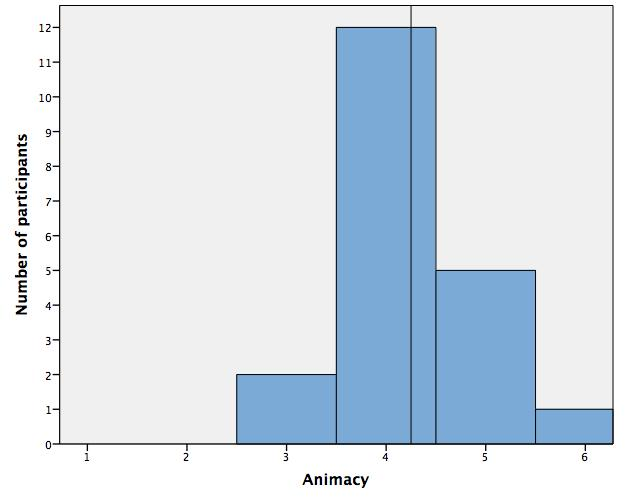
\includegraphics[width=\textwidth]{images/AnimacyBaseline.jpeg}
		\caption{Animacy histogram in the control condition. The vertical reference line marks the mean average of 4.25±0.716.}
		\label{fig:animacy_baseline}
	\end{minipage}
	\hfill
	\begin{minipage}[b]{.45\textwidth}
		\centering
		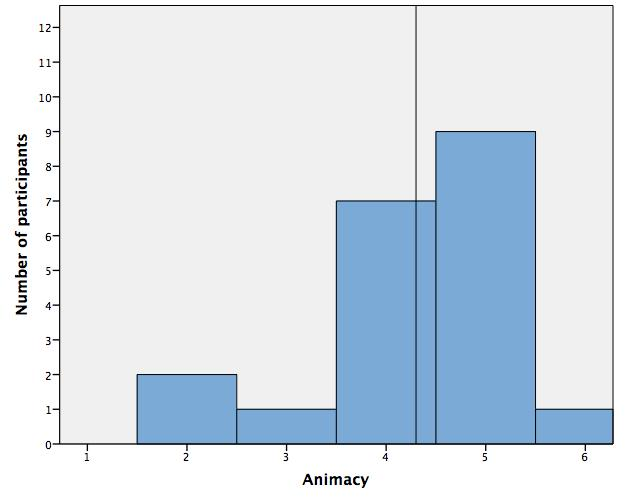
\includegraphics[width=\textwidth]{images/AnimacyRapport.jpeg}
		\caption{Animacy histogram in the rapport condition. The vertical reference line marks the mean average of 4.3±1.031.}
		\label{fig:animacy_rapport}
	\end{minipage}
\end{figure}

\textbf{Answer}: There is no definite proof that the current system improves the agent's liveness.

\subsection*{\textit{Do rapport strategies affect perceived intelligence?}}

Similar to likeability and animacy, the perceived intelligence distributions on  conditions C and R are not normal ($sig_C=0$ and $sig_R=0.002$), therefore we compare both conditions with the \textit{Mann–Whitney U} statistical test. The histograms are depicted in Figure~\ref{fig:intelligence_baseline} and Figure~\ref{fig:intelligence_rapport}, control condition and rapport condition, respectively. The histogram's shapes are dissimilar ($sig=1.0$), therefore we only compare the mean scores: 5.1±0.553 and 5.0±0.918, on conditions C and R, respectively.


\begin{figure}[H]
	\centering
	\begin{minipage}[b]{.45\textwidth}
		\centering
		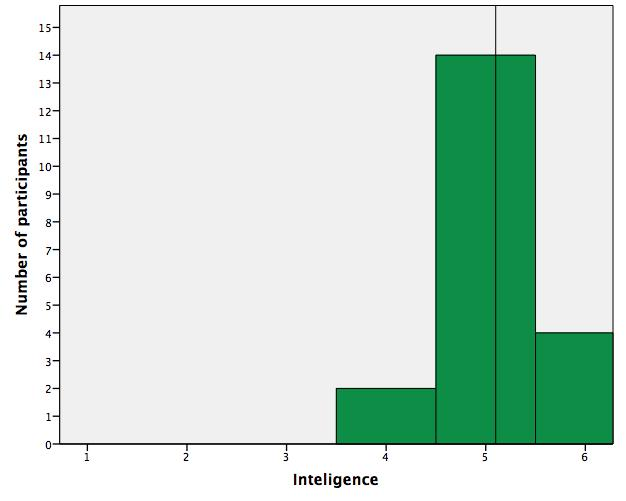
\includegraphics[width=\textwidth]{images/PerceivedIntelligenceBaseline.jpeg}
		\caption{Perceived intelligence histogram in the control condition. The vertical reference line marks the mean average of 5.1±0.553.}
		\label{fig:intelligence_baseline}
	\end{minipage}
	\hfill
	\begin{minipage}[b]{.45\textwidth}
		\centering
		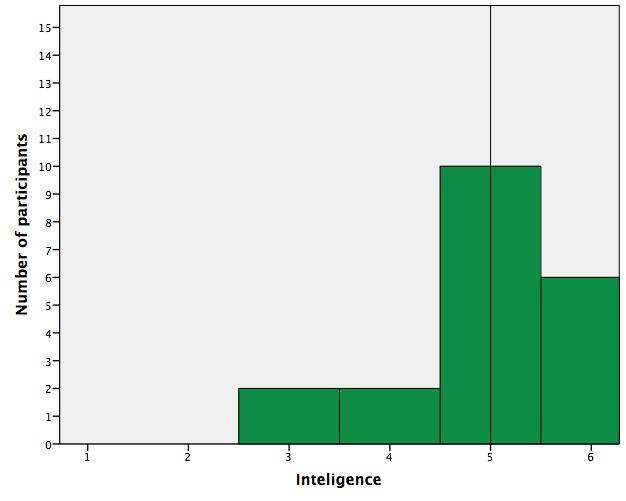
\includegraphics[width=\textwidth]{images/PerceivedIntelligenceRapport.jpeg}
		\caption{Perceived intelligence histogram in the rapport condition. The vertical reference line marks the mean average of 5.0±0.918.}
		\label{fig:intelligence_rapport}
	\end{minipage}
\end{figure}

\textbf{Answer}: There is no statistical proof that the rapport strategies have an effect on the agent's perceived intelligence.
 
\subsection*{\textit{Are the rapport strategies effective in establishing closer relationships between humans and agents?}}

In order to answer the last hypothesis, we compare the proximities answers between conditions C (Figure~\ref{fig:proximity_baseline}) and R (Figure~\ref{fig:proximity_rapport}). In both conditions, proximity follows a normal distribution ($sig_C=0.203$ and $sig_R=0.304$), therefore we use the independent \textit{t-test} statistic test which yielded the statistical significance value of 0.694 ($>0.05$), therefore we reject the null hypothesis.

\begin{figure}[H]
	\centering
	\hspace{10mm}
	\begin{minipage}[b]{.45\textwidth}
		\centering
		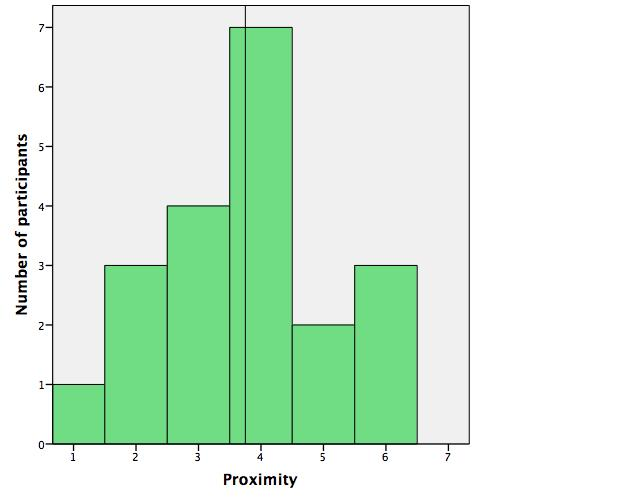
\includegraphics[width=\textwidth]{images/EmysBaseline.jpeg}
		\caption{Proximity histogram in the control condition. The vertical reference line marks the mean average of 3.75±1.410.}
		\label{fig:proximity_baseline}
	\end{minipage}
	\hfill
	\begin{minipage}[b]{.45\textwidth}
		\centering
		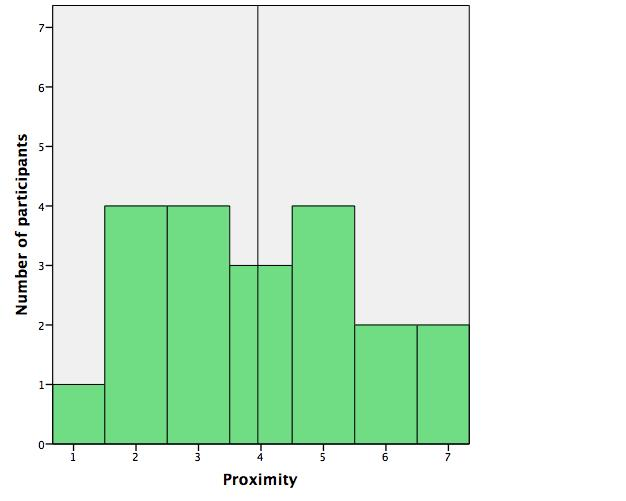
\includegraphics[width=\textwidth]{images/EmysRapport.jpeg}
		\caption{Proximity histogram in the rapport condition. The vertical reference line marks the mean average of 3.95±1.761.}
		\label{fig:proximity_rapport}
	\end{minipage}
\end{figure}

\textbf{Answer}: Despite the small increase of 0.2 on the mean score from condition C to R, the impact of the rapport strategies on proximity are inconclusive. In addition, as seen in the last bar in Figure~\ref{fig:proximity_rapport} from condition R, we had one participant that felt closest to the agent.

\section{Overall discussion}

Using mainly the subjective measures obtained from questionnaires, and given that there was no statistical significance on the obtained results, it is not possible to draw  conclusions from the experiments. However, by comparing the histograms, specially likeability’s histograms (Figure~\ref{fig:likeability_baseline} and \ref{fig:likeability_rapport}), we can infer a pattern that might lead to clear answers if we increase the sample size during future studies. Furthermore, from 1235 minutes of recorded video (using the angles illustrated in Figure~\ref{fig:quickNumbersScenario} and~\ref{fig:quickNumbersScenarioCloseup} and manual annotations during the experiments, we noticed more frequent positive reactions from the participants in the rapport condition. One one occasion, the participant remarked the agent's capability to synchronise his happy animation with its laugh. One another two independent occasions, both male and female participants flattered the agent's ability to distinguish their gender.

It is also possible to retrieve behaviour metrics by annotating (either manually or automatically) the recorded video. For example, we could compare the user's gazing behaviour between the control condition and the rapport condition, that is, compare how often the agent gazed at \ac{EMYS}. In addition, we can compare the smile frequency between both conditions using the video feed from a frontal view camera (Figure~\ref{fig:quickNumbersScenarioCloseup}).

\begin{figure}[H]
	\centering
	\frame{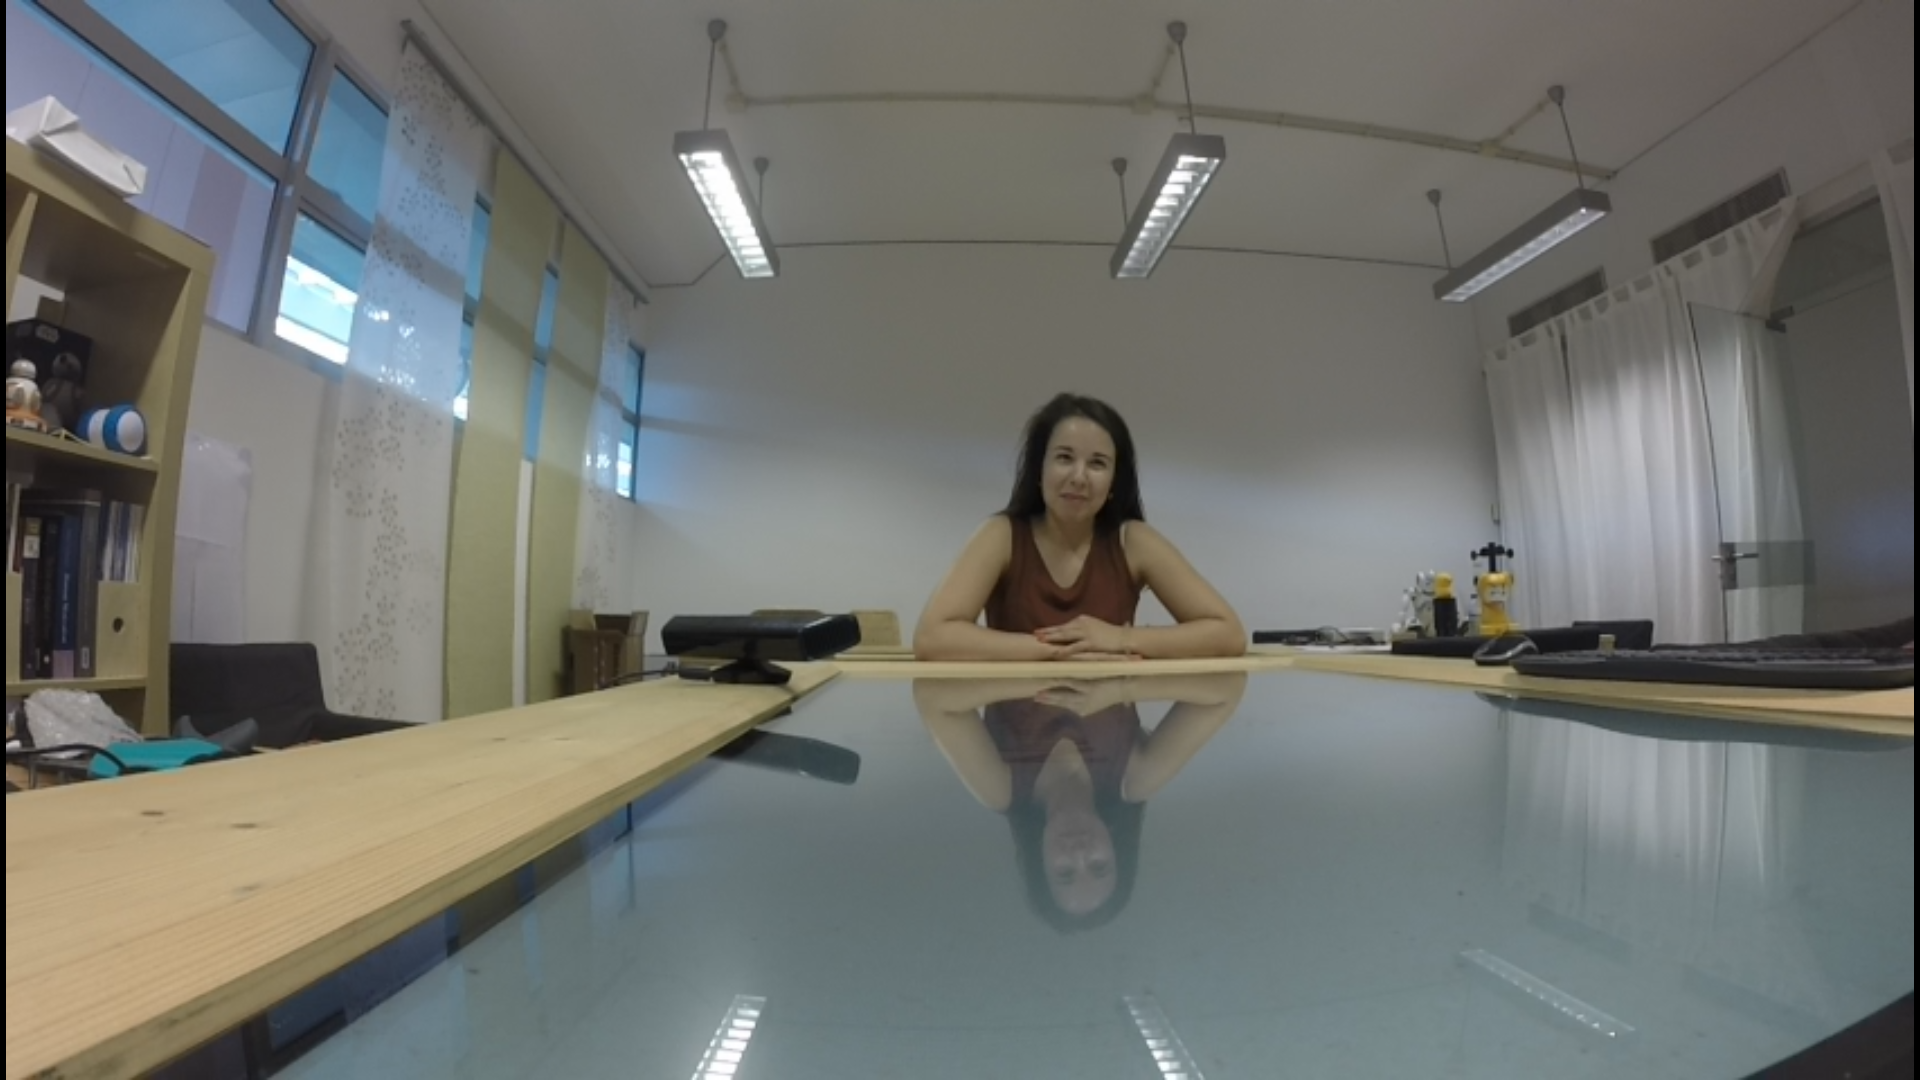
\includegraphics[width=0.7\textwidth]{images/CloseupScenario.png}}
	\caption{An example of a participation in the Quick Numbers study (frontal view).}
	\label{fig:quickNumbersScenarioCloseup}
\end{figure}

To conclude, we strongly believe that low sample size ($n=20$) and the design of the scenario were the main culprit. On one hand, with a increased sample size, the patterns might have confirmed the hypotheses with a significance lower than 5\%. And, on the other hand, the scenario should have provided more opportunities to build rapport, as even in the existing opportunities, participants were more focused on the task, and not on the agent as intended which made them less attentive to the agent's attempts to manage rapport hindering the results of the experiment. In addition, previous experience with the robot \ac{EMYS} might have the impacted on the results, as there were already attempts to build rapport in the past, with or without success. In order to reduce the impact of previous experience, the scenario should have considered different utterances considered that some participants already interacted with the partner in the past, for example, the agent might comment ``Your face is not strange to me, we already played some games in the past, didn't we?'' if the participant already interacted with \ac{EMYS} previously. This way, we are discerning between building rapport (participants who never played with \ac{EMYS} with managing rapport (participants who already played with \ac{EMYS} in the past).